\documentclass{beamer}
\usetheme{Dresden}
\usecolortheme{dolphin}
\usefonttheme[onlymath]{serif}

\usepackage[T1]{fontenc}
\usepackage[utf8]{inputenc}
\usepackage[british]{babel}
\usepackage{amsmath}
\usepackage{amsthm}
\usepackage{graphicx}
\usepackage{epstopdf}
\usepackage{subfig}
\usepackage{caption}
\usepackage{pgfplots}
\usepackage{animate}
\usepackage{bbm}
\usepackage{booktabs}
\usepackage{wrapfig}
\usepackage{listings}
\definecolor{mygray}{rgb}{0.97,0.97,0.97}
\definecolor{mygreen}{rgb}{0, 0.6, 0}
\lstset{
	backgroundcolor=\color{mygray},
	language=C++,
%	basicstyle=\scriptsize\ttfamily,
	basicstyle=\fontsize{7.5}{8.5}\selectfont\ttfamily,
	tabsize=3,
%	numbers=left,
%	numberstyle=\tiny,
%	numbersep=5pt,
%	stepnumber=5,
	breaklines=true,
	showstringspaces=false,
	keywordstyle=\color{blue},
	commentstyle=\color{mygreen},
	stringstyle=\color{red},
	keepspaces=true,
	columns=fullflexible
}

\newcommand{\code}[1]{{\footnotesize\ttfamily #1}}

%\addtobeamertemplate{navigation symbols}{}{%
%	\usebeamerfont{footline}%
%	\usebeamercolor[fg]{footline}%
%	\hspace{1em}%
%	\insertframenumber/\inserttotalframenumber
%}

\captionsetup{skip=0pt, belowskip=0pt}
\captionsetup[figure]{labelformat=empty}
\setbeamerfont{caption}{size=\scriptsize}
\pgfplotsset{every tick label/.append style={font=\tiny}}

\usecolortheme{orchid}
\setbeamercovered{transparent}

\graphicspath{{img/}}

\title
[DG-FE approximations of elliptic problems on polyhedral grids]
{Discontinuous Galerkin Finite Element approximations of elliptic problems on
polyhedral grids}
\author[Andrea Vescovini]{Andrea Vescovini}
\institute{Politecnico di Milano}
\date{11 July 2017}
%%%%%%%%%%%%%%%%%%%%%%%%%%%%%%%%%%%%%%%%%%%%%%%%%%%%%%%%%%%%%%%%%%%%%%%%%%%%
\begin{document}
\begin{frame}
	\centering
	%\includegraphics[scale=0.5]{logo}
	\maketitle
\end{frame}
%%%%%%%%%%%%%%%%%%%%%%%%%%%%%%%%%%%%%%%%%%%%%%%%%%%%%%%%%%%%%%%%%%%%%%%%%%%%
\begin{frame}{Outline}
	\tableofcontents
\end{frame}
%%%%%%%%%%%%%%%%%%%%%%%%%%%%%%%%%%%%%%%%%%%%%%%%%%%%%%%%%%%%%%%%%%%%%%%%%%%%
\section[DG methods]{Discontinuous Galerkin methods}
\begin{frame}{Model problem}
	We consider a Poisson problem with Dirichlet boundary conditions:
	\begin{equation*}\begin{cases}
		-\Delta u= f& \mbox{ in } \Omega\\
		u = g& \mbox{ on } \partial \Omega
	\end{cases}\end{equation*}
	\begin{itemize}
		\item $f \in L^2(\Omega)$.
		\item $g \in H^{1/2}(\partial \Omega)$.
		\item $\Omega \subset \mathbb{R}^3$ is a convex bounded polyhedral 		
				domain with a Lipschitz boundary $\partial \Omega$.
	\end{itemize}
	\vspace*{0.5cm}
	\centering
	We want to discretize $\Omega$ with \textbf{polyhedral elements}.
\end{frame}
%%%%%%%%%%%%%%%%%%%%%%%%%%%%%%%%%%%%%%%%%%%%%%%%%%%%%%%%%%%%%%%%%%%%%%%%%%
\begin{frame}{Definitions}
	Let $\mathcal{T}$ be a partition of	$\Omega$ into disjoint open
	polyhedral elements $\kappa$:
	\begin{itemize}
		\item The \textbf{interfaces} of $\mathcal{T}$ are the intersections of
		the two-dimensional facets of neighbouring elements.
		\item Each interface can be subdivided by a set of co-planar triangles,
		which we call \textbf{faces}.
	\end{itemize}
	\begin{figure}
		\centering
		\includegraphics[scale=0.2]{polifacce}
	\end{figure}
\end{frame}
%%%%%%%%%%%%%%%%%%%%%%%%%%%%%%%%%%%%%%%%%%%%%%%%%%%%%%%%%%%%%%%%%%%%%%%%%%
\begin{frame}{Trace Operators}
	 Let $\kappa^+$ and $\kappa^-$ be two elements sharing the face
	 $e \in \Gamma_h$ (set of internal faces), with the outward normal
	 respectively $\mathbf{n}^+$ and
	 $\mathbf{n}^-$.\\
	\begin{figure}
		\centering
		\includegraphics[scale=0.12]{polinormali}
		\end{figure}
	For every face $e \in \Gamma_h$ we define:
	\begin{align*}
	[v] = v^+ \mathbf{n}^+ + v^- \mathbf{n}^-,
	&\quad [\![ \mathbf{v} ]\!] = \mathbf{v}^+ \cdot \mathbf{n}^+ +
	\mathbf{v}^- \cdot \mathbf{n}^-,\\
	\{v\} = \frac{1}{2} (v^+ + v^-) ,
	& \quad \{\!\!\{ \mathbf{v} \}\!\!\} = \frac{1}{2} (\mathbf{v}^+
	+\mathbf{v}^-),
	\end{align*}
	that can be extended to $e \in \Gamma_D$ (set of boundary faces) through:
	\begin{equation*}
	[v] = v \mathbf{n},
	\quad [\![ \mathbf{v} ]\!] = \mathbf{v} \cdot \mathbf{n},
	\quad \{v\} = v,
	\quad \{\!\!\{ \mathbf{v} \}\!\!\} = \mathbf{v}.
	\end{equation*}
\end{frame}
%%%%%%%%%%%%%%%%%%%%%%%%%%%%%%%%%%%%%%%%%%%%%%%%%%%%%%%%%%%%%%%%%%%%%%%%%%
\begin{frame}{Variational formulation}
	We define the \textbf{broken Sobolev space}:
	\begin{equation*}
		H^s(\mathcal{T}) = \{ v \in L^2(\Omega) : v|_\kappa \in H^s(\kappa)
		\quad \forall \kappa \in \mathcal{T} \}, \quad s>0.
	\end{equation*}
	We assume that the weak solution $u \in H^s(\mathcal{T}), \; s>3/2$:
	\begin{equation*}
		\sum_{\kappa \in \mathcal{T}} \int_\kappa -\Delta u \; v
		= \sum_{\kappa \in \mathcal{T}} \bigg( \int_\kappa \nabla u \cdot
		\nabla v
		- \int_{\partial \kappa} v \nabla u \cdot \mathbf{n} \bigg) \quad
		\forall v
		\in H^s(\mathcal{T})
	\end{equation*}
	\begin{equation*}
			\sum_{\kappa \in \mathcal{T}} \int_{\partial \kappa} v \nabla u
			\cdot \mathbf{n} = ... = \sum_{e \in \Gamma} \int_e [v]
			\cdot
			\{\!\!\{
			\nabla u \}\!\!\} + \sum_{e \in \Gamma_h} \int_e [\![
			\nabla u ]\!] \{v\}
	\end{equation*}
	\begin{block}{Remark}
		$u \in H^2(\Omega) \Rightarrow [u] = 0, \; [\![\nabla u]\!] = 0 $ 
		on every internal face $e \in \Gamma_h$.
	\end{block}
\end{frame}
%%%%%%%%%%%%%%%%%%%%%%%%%%%%%%%%%%%%%%%%%%%%%%%%%%%%%%%%%%%%%%%%%%%%%%%%%%%%%%
\begin{frame}{Variational formulation}
	\begin{equation*}
	\sum_{\kappa \in \mathcal{T}} \int_\kappa \nabla u \cdot \nabla v -
	\sum_{e \in \Gamma} \int_e [v] \cdot \{\!\!\{ \nabla u \}\!\!\} =
	\sum_{\kappa \in \mathcal{T}} \int_\kappa fv \quad \forall v \in 
	H^s(\mathcal{T}).
	\end{equation*}
	We add at the left hand side two contributions:
	\begin{equation*}
		\epsilon \sum_{e \in \Gamma_h} \int_e [u] \cdot \{\!\!\{ \nabla v
		\}\!\!\}, \quad \sum_{e \in \Gamma_h} \gamma_e \int_e [u] \cdot [v],
	\end{equation*}
	and we make a \textbf{weak imposition} of Dirichlet boundary conditions 
	adding:
	\begin{equation*}
	\epsilon \sum_{e \in \Gamma_D} \int_e (u-g) \nabla v \cdot \mathbf{n}
	+ \sum_{e \in \Gamma_D} \gamma_e \int_e (u-g)v.
	\end{equation*}
\end{frame}
%%%%%%%%%%%%%%%%%%%%%%%%%%%%%%%%%%%%%%%%%%%%%%%%%%%%%%%%%%%%%%%%%%%%%%%%%%
\begin{frame}{Variational formulation}
	We introduce the bilinear form
	$a_\epsilon: H^s(\mathcal{T}) \times H^s(\mathcal{T}) \rightarrow
	\mathbb{R}$:
	\begin{multline*}
	a_\epsilon(u, v) = \sum_{\kappa \in \mathcal{T}} \int_\kappa \nabla u \cdot
	\nabla v -\\
	-\sum_{e \in \Gamma} \bigg( \int_e [v] \cdot \{\!\!\{ \nabla u \}\!\!\}
	-\epsilon \int_e [u] \cdot \{\!\!\{ \nabla v \}\!\!\}
	- \gamma_e \int_e [u]\cdot[v] \bigg)
	\end{multline*}
	and the functional $F_\epsilon: H^s(\mathcal{T}) \rightarrow \mathbb{R}$:
	\begin{equation*}
	F_\epsilon(v) = \sum_{\kappa \in \mathcal{T}} \int_\kappa fv
	+ \sum_{e \in \Gamma_D} \bigg( \epsilon \int_e g \nabla v \cdot \mathbf{n}
	+ \gamma_e \int_e gv \bigg),
	\end{equation*}
	\begin{block}{Variational formulation}
	Find $u \in H^s(\mathcal{T}), \; s>3/2$, s.t. $a_\epsilon(u, v) =
	F_\epsilon(v) \quad \forall v \in H^s(\mathcal{T})$
	\end{block}

\end{frame}
%%%%%%%%%%%%%%%%%%%%%%%%%%%%%%%%%%%%%%%%%%%%%%%%%%%%%%%%%%%%%%%%%%%%%%%%%%
\begin{frame}{Discrete formulation}
	We introduce the finite dimensional subspace of $H^s(\mathcal{T})$, $s>3/2$:
	\begin{equation*}
	\mathcal{D}_r(\mathcal{T}) = \{ v \in L^2(\Omega) : v|_\kappa \in
	\mathbb{P}_r(\kappa) \quad \forall \kappa \in \mathcal{T}  \},
	\end{equation*}
	\begin{equation*}
		|\!|v_h|\!|_{DG} = \bigg( |\!|\nabla v_h|\!|^2_{L^2(\mathcal{T})} +
		\sum_{e \in \Gamma} \gamma_e \int_e [v_h]^2 \bigg)^{1/2}.
	\end{equation*}
	\begin{block}{Discrete formulation}
	Find $u_h \in \mathcal{D}_r(\mathcal{T})$ s.t. $a_\epsilon(u_h, v_h) =
	F_\epsilon(v_h) \quad \forall v_h \in \mathcal{D}_r(\mathcal{T})$.
	\end{block}
	\begin{itemize}
		\item $\epsilon = \makebox[0.5cm][r]{$-1$} \rightarrow$ \textbf{SIPG 
		(Symmetric Interior Penalty Galerkin)}
		\item $\epsilon = \makebox[0.5cm][r]{$+1$} \rightarrow$ NIPG 
		(Non-symmetric Interior Penalty	Galerkin)
		\item $\epsilon = \makebox[0.5cm][r]{$0$} \rightarrow$ IIPG (Incomplete 
		Interior Penalty
		Galerkin)
	\end{itemize}
\end{frame}
%%%%%%%%%%%%%%%%%%%%%%%%%%%%%%%%%%%%%%%%%%%%%%%%%%%%%%%%%%%%%%%%%%%%%%%%%%%
\begin{frame}[label=main]{Grid \hyperlink{supplemental}{assumptions}}
	\begin{itemize}
	\item $\forall \kappa \in \mathcal{T}~\exists$ a set of non-overlapping 
	tetrahedra $\{T_j\}$ included in $\kappa$ s.t. each $ e \subset \partial 
	\kappa$ is shared by at least one tetrahedron $T_j$ and $\exists C > 0$ 
	s.t. $h_\kappa \leq 3C|T_j|/|e|$. 
	\item There exists a \textbf{covering} of $\mathcal{T}$ made of 
	non-overlapping	tetrahedra which we require to be regular.
	\end{itemize}
	\vspace*{0.3cm}
	In order to prove the well-posedness we choose the penalty parameter
	$\gamma_e \in L^\infty(\mathcal{T})$ such that:
	\begin{equation*} \label{eq:penalty}
	\gamma_e =
	\begin{cases}
	\sigma \max\limits_{\kappa \in \{\kappa^+, \kappa^-\}} \big\{
	\frac{r^2}{h_\kappa}\big\},
	& \quad e \in \Gamma_h, \; e \subset \partial\kappa^+ \cap
	\partial\kappa^-,\\
	\sigma\frac{r^2}{h_\kappa},& \quad e \in \Gamma_D, \; e \subset
	\partial\kappa^+ \cap \partial\Omega,
	\end{cases}
	\end{equation*}
	where $\sigma$ is a positive constant independent of $r$, $|e|$ and
	$|\kappa|$.
\end{frame}
%%%%%%%%%%%%%%%%%%%%%%%%%%%%%%%%%%%%%%%%%%%%%%%%%%%%%%%%%%%%%%%%%%%%%%%%%
\begin{frame}{Well-posedness}
	Lax-Milgram lemma $\rightarrow$ we need continuity and coercivity of the
	bilinear form $a_\epsilon (\cdot, \cdot)$ and continuity of the linear
	functional $F_\epsilon(\cdot)$.\\
	\vspace*{0.5cm}
	We exploit the following inverse trace inequality for polynomials:
	\begin{equation*}
		|\!|v|\!|^2_{L^2(\partial\kappa)} \leq C_{inv} \frac{r^2}{h_\kappa} 
		|\!|v|\!|^2_{L^2(\kappa)} \quad \forall v \in \mathbb{P}_r(\kappa).
	\end{equation*}
	where $C_{inv}$ is a constant independent of $|\kappa|$, $r$ and $v$.\\
	\vspace*{0.5cm}
	We conclude that we need the constant $\sigma$ of the penalization 
	parameter $\gamma_e$ to be large enough.
\end{frame}
%%%%%%%%%%%%%%%%%%%%%%%%%%%%%%%%%%%%%%%%%%%%%%%%%%%%%%%%%%%%%%%%%%%%%%%%%%%
\begin{frame}{Error estimates}
	\begin{theorem}
		Suppose that assumptions on the grid hold and let
		$u_h \in \mathcal{D}_r(\mathcal{T})$ be the DG solution of
		the discrete formulation. If the exact solution $u$ belongs to
		$H^k(\mathcal{T}), \; k>5/2$, s.t.
		$\mathcal{E}v|_\mathcal{K}\in H^k(\mathcal{K}) \quad \forall
		\kappa\in\mathcal{T}$, where $\kappa~\subset~\mathcal{K}, \;
		\mathcal{K}~\in~\mathcal{T}^\#$, then the following bounds hold:
		\begin{equation*}
			|\!|u-u_h|\!|_{DG} \leq G \frac{h^{s-1}}{r^{k-3/2}}
			|\!|u|\!|_{H^s(\Omega)},
		\end{equation*}
		\begin{equation*}
		|\!|u-u_h|\!|_{L^2(\Omega)} \leq C_{L^2} \frac{h^s}{r^{k-1}}
		|\!|u|\!|_{H^s(\Omega)},
		\end{equation*}
		where $s = \min \{r+1, k\}$ and the constants $G$, $C_{L^2}$ are
		independent of the discretization parameters.
	\end{theorem}
\end{frame}
%%%%%%%%%%%%%%%%%%%%%%%%%%%%%%%%%%%%%%%%%%%%%%%%%%%%%%%%%%%%%%%%%%%%%%%%%%%
\section{Implementation details}
\begin{frame}{Basis functions}
	\begin{itemize}
		\item $\forall \kappa \in \mathcal{T}$ construct a Cartesian bounding 
		box $B_\kappa=I_1\times I_2 \times I_3$ such that $\bar{\kappa} \subseteq 
		\bar{B_\kappa}$.
		\pause
		\item Define $\mathbb{P}_r(B_\kappa)$ spanned by basis
		functions $\{ \phi_{i,\kappa} \}_{i=1}^{dim(\mathbb{P}_r(B_\kappa))}$.
	\end{itemize}
	We choose tensor product Legendre polynomials as basis over $B_\kappa$:
	\begin{equation*}
		\phi_{\kappa,i}(\mathbf{x}) =
		L_{r_1}^{[I_1]}(x)L_{r_2}^{[I_2]}(y)L_{r_3}^{[I_3]}(z), \quad
		r_1+r_2+r_3 \leq r,
	\end{equation*}
	where $L_r^{[I_b]}$ is a Legendre polynomial scaled over the interval $I_b$:
	\begin{equation*}
	L_r^{[I_b]} (x) = \frac{1}{\sqrt{h_b}} L_r \bigg( \frac{x-m_b}{h_b} \bigg),
	\quad h_b = \frac{x_2-x_1}{2}, \quad m_b=\frac{x_1+x_2}{2}.
	\end{equation*}
	\pause
	\begin{itemize}
		\item Restrict the support of $\phi_{\kappa, i}(\mathbf{x}), \;
		i=1,\dots,dim(\mathbb{P}_r(B_\kappa))$ to $\kappa$.
	\end{itemize}
\end{frame}
%%%%%%%%%%%%%%%%%%%%%%%%%%%%%%%%%%%%%%%%%%%%%%%%%%%%%%%%%%%%%%%%%%%%%%%%%%%
\begin{frame}{Matrix assembly}
	We expand the solution $u_h$ in basis functions and we get the
	algebraic formulation: find $\mathbf{u} = [u_1, \dots, u_{N_h}]^T \in
	\mathbb{R}^{N_h} $ such that:
	\begin{equation*}
	\mathrm{A}\mathbf{u} = \mathbf{f},
	\end{equation*}
	where $\mathrm{A} \in \mathbb{R}^{N_h \times N_h}, \; \mathrm{A}_{ij} =
	a(\phi_j, \phi_i)$ and $\mathbf{f} \in \mathbb{R}^{N_h}, \; \mathbf{f}_i =
	F(\phi_i)$.\\
	%\vspace*{0.4cm}
	%The matrix $\mathrm{A}$ is the sum of four matrices:
	\begin{equation*}
	\mathrm{A} =
	\mathrm{V} - \mathrm{I} - \mathrm{I}^T + \mathrm{S}
	\end{equation*}
	\begin{itemize}
		\item $\mathrm{V}_{ij} = \sum\limits_{\kappa \in \mathcal{T}}
		\int_\kappa
		\nabla \phi_j \cdot \nabla \phi_i, \quad i,j=1,\dots,N_h$
		\item $\mathrm{I}_{ij} = \sum\limits_{e \in \Gamma} \int_e
		[\![\phi_j]\!]
		\cdot \{\!\!\{ \nabla \phi_i \}\!\!\}, \quad i,j=1,\dots,N_h$
		\item $\mathrm{S}_{ij} = \sum\limits_{e \in \Gamma} \gamma_e \int_e
		[\![
		\phi_j ]\!] \cdot [\![ \phi_i ]\!], \quad i,j=1,\dots,N_h$
	\end{itemize}
\end{frame}
%%%%%%%%%%%%%%%%%%%%%%%%%%%%%%%%%%%%%%%%%%%%%%%%%%%%%%%%%%%%%%%%%%%%%%%%%%%
\begin{frame}{Sparsity pattern}
	\vspace*{-12pt}
	\begin{align*}
	\mathrm{I} \rightarrow \int_e [\![\phi_j]\!] \cdot \{\!\!\{ \nabla \phi_i
	\}\!\!\} &=
	\frac{1}{2} \int_e (\nabla{\phi_i}^+ \cdot \mathbf{n}^+ )\phi_j^+
	+ \frac{1}{2} \int_e (\nabla{\phi_i}^- \cdot \mathbf{n}^- )\phi_j^-\\
	&- \frac{1}{2} \int_e (\nabla{\phi_i}^+ \cdot \mathbf{n}^+ )\phi_j^-
	- \frac{1}{2} \int_e (\nabla{\phi_i}^- \cdot \mathbf{n}^- )\phi_j^+
	\end{align*}
	\vspace*{-1cm}
	\begin{minipage}[t]{0.55\textwidth}
		\begin{multline*}
			\mathrm{S} \rightarrow \gamma_e \int_e [\![\phi_j]\!] \cdot
			[\![\phi_i]\!] =\\
			\gamma_e \int_e \phi_i^+ \phi_j^+
			+ \gamma_e \int_e \phi_i^- \phi_j^-\\
			- \gamma_e \int_e \phi_i^+ \phi_j^-
			- \gamma_e \int_e \phi_i^- \phi_j^+
		\end{multline*}
	\end{minipage}%%%%%%%%%%%%%%%%
	\begin{minipage}[t]{0.45\textwidth}
	\begin{figure}
		\centering
		\includegraphics[scale=0.35]{spy_A}\\
		\tiny
		\textit{Sparsity pattern of $\mathrm{A}$ computed over a mesh
		of 392 polyhedral elements and $r=2$}.
	\end{figure}
\end{minipage}
\end{frame}
%%%%%%%%%%%%%%%%%%%%%%%%%%%%%%%%%%%%%%%%%%%%%%%%%%%%%%%%%%%%%%%%%%%%%%%%%%%
\begin{frame}{Quadrature rules}
	\begin{itemize}
		\item Construct a sub-triangulation.
		\item Exploit standard integration schemes.
	\end{itemize}
	For example let	$\kappa_\mathcal{S} = \{\tau_\kappa\}$ be a non-overlapping
	sub-triangulation for the element $\kappa$ made of tetrahedra:
	\begin{multline*}
	\int_\kappa \nabla u \cdot \nabla v = \sum_{\tau_\kappa \in
	\kappa_\mathcal{S}} \nabla u \cdot \nabla v \approx\\
	\approx \sum_{\tau_\kappa \in
	\kappa_\mathcal{S}} \sum_{i=1}^{q} \nabla u(F_\kappa(\xi_i)) \cdot \nabla
	v(F_\kappa(\xi_i)) det(J_{F_\kappa}(\xi_i))w_i,
	\end{multline*}
	where $F_\kappa: \hat{\kappa} \rightarrow \tau_\kappa$ is the map from the
	reference simplex $\hat{\kappa}$ to $\tau_\kappa$ and $(\xi_i,
	w_i)^q_{i=1}$ denote the quadrature nodes and weights
	over $\hat{\kappa}$.
\end{frame}
%%%%%%%%%%%%%%%%%%%%%%%%%%%%%%%%%%%%%%%%%%%%%%%%%%%%%%%%%%%%%%%%%%%%%%%%%%%
\section{The C++ library}
\begin{frame}{PolyDG}
We developed a C++ library, called PolyDG, to test the method that has been 
presented.\\
\vspace{0.5cm}
The workflow of the code can be split into:
\begin{itemize}
	\item \makebox[3cm][l]{\emph{Geometrical} level} $ \rightarrow $ class \code{Mesh}
	\item \makebox[3cm][l]{\emph{Functional} level} $ \rightarrow $ class \code{FeSpace}
	\item \makebox[3cm][l]{\emph{Problem} level} $ \rightarrow $ class \code{Problem}
\end{itemize}
\vspace{0.5cm}
 The library Eigen was used for linear algebra.
\end{frame}
%%%%%%%%%%%%%%%%%%%%%%%%%%%%%%%%%%%%%%%%%%%%%%%%%%%%%%%%%%%%%%%%%%%%
\begin{frame}{The class Mesh}
\begin{columns}
\begin{column}{0.55\textwidth}
\lstinputlisting[lastline=17]{code/Mesh.hpp}
\end{column}
\begin{column}{0.55\textwidth}
\lstinputlisting[firstline=18]{code/Mesh.hpp}
\end{column}
\end{columns}
\end{frame}
%%%%%%%%%%%%%%%%%%%%%%%%%%%%%%%%%%%%%%%%%%%%%%%%%%%%%%%%%%%%%%%%%
\begin{frame}{The class FeSpace}
\begin{columns}
	\begin{column}{0.57\textwidth}
		\lstinputlisting[lastline=17]{code/FeSpace.hpp}
	\end{column}
	\begin{column}{0.57\textwidth}
		\lstinputlisting[firstline=18]{code/FeSpace.hpp}
	\end{column}
\end{columns}
\end{frame}
%%%%%%%%%%%%%%%%%%%%%%%%%%%%%%%%%%%%%%%%%%%%%%%%%%%%%%%%%%%%%%%%
%%%%%%%%%%%%%%%%%%%%%%%%%%%%%%%%%%%%%%%%%%%%%%%%%%%%%%%%%%%%
\begin{frame}{Quadrature formulas}
\begin{columns}
	\begin{column}{0.57\textwidth}
		\lstinputlisting[lastline=11]{code/QuadRuleManager.hpp}
	\end{column}
	\begin{column}{0.57\textwidth}
		\lstinputlisting[firstline=13]{code/QuadRuleManager.hpp}
	\end{column}
\end{columns}
	\lstinputlisting[lastline=8]{code/FeSpace.cpp}
\end{frame}
%%%%%%%%%%%%%%%%%%%%%%%%%%%%%%%%%%%%%%%%%%%%%%%%%%%%%%%%%%
\begin{frame}{The class Problem}
%		\lstinputlisting[lastline=19]{code/Problem.hpp}
%		\lstinputlisting[firstline=33, lastline=46]{code/Problem.hpp}
\begin{columns}
	\begin{column}{0.82\textwidth}
		\lstinputlisting[lastline=22]{code/Problem_slides.hpp}
	\end{column}
	\begin{column}{0.28\textwidth}
		\lstinputlisting[firstline=24]{code/Problem_slides.hpp}
	\end{column}
\end{columns}
\end{frame}
%%%%%%%%%%%%%%%%%%%%%%%%%%%%%%%%%%%%%%%%%%%%%%%%%%%%%%%
\begin{frame}[fragile]{Integration}
\begin{lstlisting}
Problem poisson(Vh); // Vh is a FeSpace
GradPhiJ uGrad;
GradPhiI vGrad;
poisson.integrateVol(dot(uGrad, vGrad), true);
\end{lstlisting}
\lstinputlisting[firstline=48]{code/Problem.hpp}
\end{frame}
%%%%%%%%%%%%%%%%%%%%%%%%%%%%%%%%%%%%%%%%%%%%%%%%%%%%%%%%%
\begin{frame}{Expression templates}
\lstinputlisting{code/ExprWrapper_slides.hpp}
\pause
\lstinputlisting{code/BinaryOperator_slides.hpp}
\end{frame}
%%%%%%%%%%%%%%%%%%%%%%%%%%%%%%%%%%%%%%%%%%%%%%%%%%%%%%%%%%
\begin{frame}[fragile]{Expression templates}
\lstinputlisting{code/GradPhiJ_slides.hpp}
\pause
\begin{lstlisting}
poisson.integrateVol(dot(uGrad, vGrad), true);
poisson.integrateFacesInt(-dot(uGradAver, vJump) - dot(uJump, vGradAver) + gamma * dot(uJump, vJump), true);
poisson.integrateFacesExt(-dot(uGradAver, vJump) - dot(uJump, vGradAver) + gamma * dot(uJump, vJump), dirichlet, true);
poisson.integrateVolRhs(f * v);
poisson.integrateFacesExtRhs(-gd * dot(n, vGrad) + gamma * gd * v, dirichlet);

poisson.finalizeMatrix();
\end{lstlisting}
\end{frame}
%%%%%%%%%%%%%%%%%%%%%%%%%%%%%%%%%%%%%%%%%%%%%%%%%%%%%%%%%%
\begin{frame}{Solvers and post processing}
\begin{columns}
	\begin{column}{1.15\textwidth}
\lstinputlisting[firstline=21, lastline=31, caption=inside the class 
Problem]{code/Problem.hpp}
\end{column}
\end{columns}
\end{frame}
%%%%%%%%%%%%%%%%%%%%%%%%%%%%%%%%%%%%%%%%%%%%%%%%%%%%%%%%%%%%%%%%%%%%%%%%%
\section{Numerical results}
\begin{frame}{Numerical results}
	We test the method choosing $\Omega = (0,1)^3$, $u(x,y,z) = e^{xyz}$,
	$\sigma = 10$.
	\begin{figure}
		\centering
		\subfloat[Polyhedral mesh consisting of 15 elements.]
		{\includegraphics[width=.45\textwidth]{mesh_48p}}
		\quad
		\subfloat[Solution computed over a polyhedral mesh.]
		{\includegraphics[width=.45\textwidth]{solution_3072p}}
	\end{figure}
\end{frame}
%%%%%%%%%%%%%%%%%%%%%%%%%%%%%%%%%%%%%%%%%%%%%%%%%%%%%%%%%%%%%%%%%%%%%%%%%%%%
\begin{frame}{$h$-convergence}
	\begin{itemize}
		\item Tetrahedral, hexahedral, mixed tetrahedral/hexahedral and
		polyhedral meshes.
		\item $r = 1,2,3$.
		\item $L^2$-norm and $H^1$-seminorm of the error $e_h = u - u_h$.
	\end{itemize}

	\begin{table} \tiny
		\centering
		\[
		\begin{array}{ccccccc}
		\toprule
		r & \text{Error} & \text{28 elem} & \text{224 elem} & \text{756 elem} &
		\text{1792 elem} & \text{Rate} \\
		\midrule
		2 & |\!|\nabla e_{h}|\!|_{L^2} & 7.4183 \times 10^{-2} & 1.9944 \times
		10^{-2} & 8.9959 \times 10^{-3} & 5.0984 \times 10^{-3} & 1.9738\\
		& |\!|e_{h}|\!|_{L^2} & 4.1276 \times 10^{-3} & 7.0478 \times 10^{-4} &
		2.1079 \times 10^{-4} &
		8.9470 \times 10^{-5} & 2.9787\\
		\bottomrule
		\end{array}
		\]
		\caption{\textit{Computed errors on a sequence of mixed
		tetrahedral/hexahedral meshes.}}
%	\end{table}
%\begin{table} \tiny
%	\centering
	\[
	\begin{array}{ccccccc}
	\toprule
	r & \text{Error} & \text{15 elem} & \text{120 elem} & \text{392 elem} &
	\text{965 elem} & \text{Rate} \\
	\midrule
	2 & |\!|\nabla e_{h}|\!|_{L^2} & 8.7963 \times 10^{-2} & 4.2298 \times
	10^{-2} & 2.3058 \times 10^{-2} & 1.3036 \times 10^{-2} & 1.9823\\
	& |\!|e_{h}|\!|_{L^2} & 5.3520 \times 10^{-3} & 1.8324 \times 10^{-3} &
	7.5865 \times 10^{-4} & 2.8963 \times 10^{-4} & 3.3472\\
	\bottomrule
	\end{array}
	\]
	\caption{\textit{Computed errors on a sequence of polyhedral meshes..}}
\end{table}

\end{frame}
%%%%%%%%%%%%%%%%%%%%%%%%%%%%%%%%%%%%%%%%%%%%%%%%%%%%%%%%%%%%%%%%%%%%%%%%%%%
\begin{frame}{Comparison with other methods}
	Comparison with:
	\begin{itemize}
		\item Classical SIPG method, based on a Lagrange polynomial basis.
		\item Standard continuous Galerkin finite element method.
	\end{itemize}
	\vspace*{-0.7cm}
\begin{figure}[h!]
	\centering
	\subfloat[][$r=1$, $|\!|\nabla e_h|\!|_{L^2(\mathcal{T})}$] {
		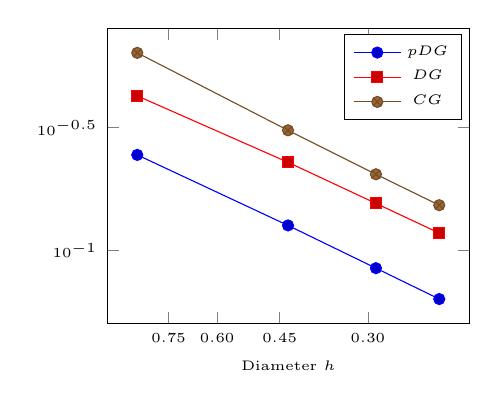
\begin{tikzpicture}
		\begin{loglogaxis}[width=0.51\textwidth,
		xlabel style={font=\tiny}, xlabel=Diameter $h$, x 
		dir=reverse, 
		xtick={0.30,0.45,0.60, 0.75}, 
		xticklabels={$0.30$,$0.45$,$0.60$,$0.75$}, legend style={font=\tiny}]
		\addplot coordinates
		{(0.866, 2.4486e-1) (0.433, 1.2628e-1) (0.289, 8.4537e-2) (0.216, 6.3263e-2)};
		\addlegendentry{$pDG$}
		\addplot coordinates
		{(0.866, 4.2617e-1) (0.433, 2.2842e-1) (0.289, 1.5530e-1) (0.216, 
		1.1752e-1)};
		\addlegendentry{$DG$}
		\addplot coordinates
		{(0.866, 6.3842e-1) (0.433, 3.0849e-1) (0.289, 2.0414e-1) (0.216, 
		1.5270e-1)};
		\addlegendentry{$CG$}
		\end{loglogaxis}
		\end{tikzpicture}}
	\subfloat[$r=1$, $|\!|e_h|\!|_{L^2(\mathcal{T})}$]{
		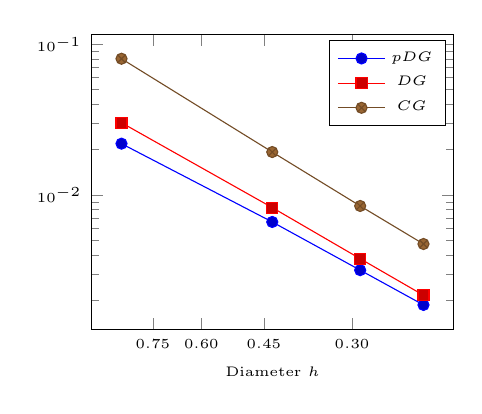
\begin{tikzpicture}
		\begin{loglogaxis}[width=0.51\textwidth, xlabel style={font=\tiny}, 
		xlabel=Diameter $h$, x dir=reverse, 
		xtick={0.30,0.45,0.60, 0.75}, 
		xticklabels={$0.30$,$0.45$,$0.60$,$0.75$}, legend style={font=\tiny}]
		\addplot coordinates
		{(0.866, 2.1925e-2) (0.433, 6.6318e-3) (0.289, 3.1769e-3) (0.216, 1.8679e-3)};
		\addlegendentry{$pDG$}
		\addplot coordinates
		{(0.866, 3.0189e-2) (0.433, 8.2593e-3) (0.289, 3.7849e-3) (0.216, 
		2.1654e-3)};
		\addlegendentry{$DG$}
		\addplot coordinates
		{(0.866, 8.0221e-2) (0.433, 1.9297e-2) (0.289, 8.4678e-3) (0.216, 
		4.7368e-3)};
		\addlegendentry{$CG$}
		\end{loglogaxis}
		\end{tikzpicture}}
	\end{figure}
\end{frame}
%%%%%%%%%%%%%%%%%%%%%%%%%%%%%%%%%%%%%%%%%%%%%%%%%%%%%%%%%%%%%%%%%%%%%%%%%%
\begin{frame}{$r$-convergence}
	\begin{itemize}
		\item Tetrahedral, hexahedral, mixed tetrahedral/hexahedral and
		polyhedral meshes.
		\item $r = 1,2,3,4,5$.
		\item $L^2$-norm and $H^1$-seminorm of the error $e_h = u - u_h$.
	\end{itemize}
	\vspace*{-0.7cm}
	\begin{figure}
		\subfloat[Tet/hex elements.]{
			\begin{tikzpicture}
			\begin{semilogyaxis}[width=0.55\textwidth, height=0.55\textheight,
			xlabel style={font=\tiny}, xlabel={Basis degree}, xtick={1,2,3,4,5}, ytick={1e-2, 1e-5, 1e-8},
			legend style={font=\tiny}]
			\addplot coordinates
			{(1, 5.50185e-2) (2, 5.09841e-3) (3, 3.15288e-4) (4,1.74089e-5) (5,1.08802e-6)};
			\addlegendentry{$|\!|\nabla e_{h}|\!|_{L^2}$}
			\addplot coordinates
			{(1, 1.35461e-3) (2, 8.947e-5) (3, 4.04412e-6) (4, 1.9446e-7) (5,9.37969e-9)};
			\addlegendentry{$|\!|e_{h}|\!|_{L^2}$}
			\end{semilogyaxis}
			\end{tikzpicture}}
		\subfloat[Polyhedral elements.]{
			\begin{tikzpicture}
			\begin{semilogyaxis}[width=0.55\textwidth, height=0.55\textheight,
			xlabel style={font=\tiny}, xlabel={Basis degree},
			xtick={1,2,3,4,5}, legend style={font=\tiny}]
			\addplot coordinates
			{(1, 1.1807e-1) (2, 1.30364e-2) (3, 1.12395e-3) (4, 8.32443e-5) (5, 1.00171e-5 )};
			\addlegendentry{$|\!|\nabla e_{h}|\!|_{L^2}$}
			\addplot coordinates
			{(1, 5.6298e-3) (2, 2.89633e-4) (3, 2.03593e-5) (4, 1.34948e-6) (5, 9.12435e-8)};
			\addlegendentry{$|\!|e_{h}|\!|_{L^2}$}
			\end{semilogyaxis}
			\end{tikzpicture}}
	\end{figure}
\end{frame}
%%%%%%%%%%%%%%%%%%%%%%%%%%%%%%%%%%%%%%%%%%%%%%%%%%%%%%%%%%%%%%%%%%%%%%%%%%%
% \begin{frame}{$r$-convergence}
% 	\vspace*{-0.5cm}
% 	\begin{figure}[h]
% 		\centering
% 		\subfloat[][Tetrahedral elements.]{
% 			\begin{tikzpicture}
% 			\begin{semilogyaxis}[width=0.55\textwidth, height=0.4\textheight,
% 			xlabel near ticks, xlabel style={font=\tiny}, xlabel={Basis
% 				degree}, xtick={1,2,3},
% 			legend style={font=\tiny}]
% 			\addplot coordinates
% 			{(1, 9.9471e-2) (2, 4.6327e-3) (3, 2.0627e-4)};
% 			\addlegendentry{$|\!|\nabla e_{h}|\!|_{L^2}$}
% 			\addplot coordinates
% 			{(1, 1.0227e-3) (2, 9.4460e-5) (3, 3.6715e-6)};
% 			\addlegendentry{$|\!|e_{h}|\!|_{L^2}$}
% 			\end{semilogyaxis}
% 			\end{tikzpicture}}
% 		\subfloat[][Hexahedral elements.]{
% 			\begin{tikzpicture}
% 			\begin{semilogyaxis}[width=0.55\textwidth, height=0.4\textheight,
% 			xlabel near ticks, xlabel style={font=\tiny}, xlabel={Basis
% 				degree},
% 			xtick={1,2,3},
% 			legend style={font=\tiny}]
% 			\addplot coordinates
% 			{(1, 8.4123e-2) (2, 4.6362e-3) (3, 2.5782e-4)};
% 			\addlegendentry{$|\!|\nabla e_{h}|\!|_{L^2}$}
% 			\addplot coordinates
% 			{(1, 1.8931e-3) (2, 7.9122e-5) (3, 3.6604e-6)};
% 			\addlegendentry{$|\!|e_{h}|\!|_{L^2}$}
% 			\end{semilogyaxis}
% 			\end{tikzpicture}}\\
% 		\vspace*{-0.4cm}
% 		\subfloat[][Tet/hex elements.]{
% 			\begin{tikzpicture}
% 			\begin{semilogyaxis}[width=0.55\textwidth, height=0.4\textheight,
% 			xlabel near ticks, xlabel style={font=\tiny}, xlabel={Basis
% 			degree},
% 			xtick={1,2,3},
% 			legend style={font=\tiny}]
% 			\addplot coordinates
% 			{(1, 9.4090e-2) (2, 5.0984e-3) (3, 2.7689e-4)};
% 			\addlegendentry{$|\!|\nabla e_{h}|\!|_{L^2}$}
% 			\addplot coordinates
% 			{(1, 1.4851e-3) (2, 8.9470e-5) (3, 3.9958e-6)};
% 			\addlegendentry{$|\!|e_{h}|\!|_{L^2}$}
% 			\end{semilogyaxis}
% 			\end{tikzpicture}}
% 		\subfloat[][Polyhedral elements.]{
% 			\begin{tikzpicture}
% 			\begin{semilogyaxis}[width=0.55\textwidth, height=0.4\textheight,
% 			xlabel near ticks, xlabel style={font=\tiny}, xlabel={Basis
% 				degree}, xtick={1,2,3},
% 			legend style={font=\tiny}]
% 			\addplot coordinates
% 			{(1, 1.4168e-1) (2, 1.3036e-2) (3, 1.1137e-3)};
% 			\addlegendentry{$|\!|\nabla e_{h}|\!|_{L^2}$}
% 			\addplot coordinates
% 			{(1, 5.9973e-3) (2, 2.8963e-4) (3, 2.0407e-5)};
% 			\addlegendentry{$|\!|e_{h}|\!|_{L^2}$}
% 			\end{semilogyaxis}
% 			\end{tikzpicture}}
% 		\label{fig:rconv}
% 	\end{figure}
% \end{frame}
%%%%%%%%%%%%%%%%%%%%%%%%%%%%%%%%%%%%%%%%%%%%%%%%%%%%%%%%%%%%%%%%%%%%%%%%%%%%%%%%
\begin{frame}{Conclusions}
	\begin{itemize}
		\item Great flexibility in handling general meshes.
		\item Many degrees of freedom.
		\item Fewer elements to discretize complicated geometries.
		\item ET implementation allows a simple interface and it is performing.
	\end{itemize}
	Future improvements:
	\begin{itemize}
		\item Improve linear system solvers.
		\item Parallelization.
	\end{itemize}
\end{frame}
%%%%%%%%%%%%%%%%%%%%%%%%%%%%%%%%%%%%%%%%%%%%%%%%%%%%%%%%%%%%%%%%%%%%%%%%%%%%%%%%
\begin{frame}{Main references}
\begin{itemize}
%	\item Antonietti, Cangiani, Collins, Dong, Georgoulis, Giani, Houston: 
%	Review of discontinuous Galerkin finite element methods for partial 
%	differential equations on complicated domains (2016).
	
	\item Antonietti, Houston, Hu, Sarti, Verani: Multigrid
	algorithms for hp-version interior penalty discontinuous Galerkin methods
	on polygonal and polyhedral meshes (2017).
	
	\item Cangiani, Georgoulis, Houston: Hp-Version discontinuous
	Galerkin methods on polygonal and polyhedral meshes (2014).
	
	\item Di Pietro, Veneziani: Expression templates implementation of continuous and discontinuous Galerkin methods (2009).
	
	\item Quarteroni: Numerical Models for Differential Problems (2014).
	
	\item Rivière: Discontinuous Galerkin Methods for Solving Elliptic and
		Parabolic Equations: Theory and Implementation (2008).
		
\end{itemize}
\end{frame}
%%%%%%%%%%%%%%%%%%%%%%%%%%%%%%%%%%%%%%%%%%%%%%%%%%%%%%%%%%%%%%%%%%%%%%%%%%%%%%%
\appendix
\begin{frame}[label=supplemental]{Appendix}{Assumptions of the polyhedral
grid}
	\begin{block}{Assumption 1}
		Given $\kappa \in \mathcal{T}$, there exists a set of non-overlapping
		(not
		necessarily shape-regular) three-dimensional simplices $T_j \subset
		\kappa,
		\; j = 1,\dots, n_\kappa$, such that for any face $e \subset \partial
		\kappa$, $\bar{e} = \partial \bar{\kappa} \cap \partial \bar{T_j}$, for
		some $j$,
		\begin{equation*}
		\cup_{j = 1}^{n_\kappa} \bar{T_k} \subseteq \bar{\kappa},
		\end{equation*}
		and  $\exists C > 0$ such that the diameter $h_\kappa$ of $\kappa$ can
		be bounded by:
		\begin{equation*}
		h_\kappa \leq C \frac{3 |T_j|}{|e|} \quad \forall j = 1,\dots,n_\kappa.
		\end{equation*}
	\end{block}
\end{frame}
%%%%%%%%%%%%%%%%%%%%%%%%%%%%%%%%%%%%%%%%%%%%%%%%%%%%%%%%%%%%%%%%%%%%%%%%%%%%%%%
\begin{frame}{Appendix}
	\begin{block}{Assumption 2}
		Let $\mathcal{T}^\# = \{ \mathcal{K} \}$ be a covering of $\Omega$ made
		of shaped-regular three-dimensional simplices $\mathcal{K}$. We assume
		that for any $\kappa\in\mathcal{T} \quad
		\exists\mathcal{K}\in\mathcal{T}^\#$
		such that $\kappa\subset\mathcal{K}$, that $\exists~C_d>0$ such that:
		\begin{equation*}
			diam(\mathcal{K})\leq~C_dh_\kappa, \quad \text{uniformly with
			respect to the mesh size}
		\end{equation*}
		and that $\exists~C_c>0$ such that:
		\begin{equation*}
			\max\limits_{\kappa \in \mathcal{T}} card \big\{ \kappa' \in
			\mathcal{T} : \kappa' \cap \mathcal{K} \ne \emptyset, \;
			\mathcal{K} \in \mathcal{T}^\# \text{ such that } \kappa \subset
			\mathcal{K} \big\} \leq C_c.
		\end{equation*}
	\end{block}
%	\vspace*{-0.5cm}
%	\begin{block}{Assumption 3}
%		The mesh $\mathcal{T}$ is quasi uniform, i.e. $\exists C>0$ such that
%		$h~\leq~C \min_{\kappa \in \mathcal{T}} h_\kappa$.
%	\end{block}
\end{frame}
\end{document}
